\documentclass[11pt]{article}
\usepackage[margin=1in]{geometry}
\usepackage{amsmath,amssymb,bm}
\usepackage{graphicx}
\usepackage{booktabs}
\usepackage{subcaption}
\usepackage{enumitem}
\usepackage{xcolor}
\usepackage{listings}
\usepackage[colorlinks=true,linkcolor=blue,urlcolor=blue]{hyperref}

\graphicspath{{../code/figs/}}

\newcommand{\pib}{\pi_b}
\newcommand{\Ahat}{\hat{A}}
\newcommand{\Qbar}{\bar{Q}}
\newcommand{\E}{\mathbb{E}}
\newcommand{\Ehat}{\hat{\mathbb{E}}}
\newcommand{\code}[1]{\texttt{#1}}
\newcommand{\RESULT}[1]{\textcolor{red}{[RESULT: #1]}}

\lstset{basicstyle=\ttfamily\small, columns=fullflexible, breaklines=true, frame=single}

\title{ECE 562 Assignment 4: Soft Actor-Critic}
\author{Emmanuel Oluwasegun Olateju (\href{mailto:eolateju@ualberta.ca}{eolateju@ualberta.ca})}
\date{\today}

\begin{document}
\maketitle

%=====================================================================
\section*{Section 1: Implementing SAC}

\subsection*{Output of \code{python test\_sac.py}}
\lstinputlisting{../code/test_output.txt}

\subsection*{Q1: The tanh-squashed Gaussian policy (\code{networks.py}, TODO 1)}
\begin{itemize}
  \item Build \code{Normal(mu, log\_std.exp())} and draw $u$ with \code{rsample()}, so that
        $u=\mu_\theta(s)+\sigma_\theta(s)\odot\xi$ and gradients flow from $u$ back to $\theta$.
  \item The action is $a=\tanh(u)$.
  \item $\log\mathcal N_\theta(u\mid s)$ is \code{log\_prob(u).sum(-1)} (sum over the 3 action dimensions),
        and $\log\pi_\theta(a\mid s)=\log\mathcal N_\theta(u\mid s)-\code{tanh\_log\_det\_jacobian(u)}$.
        Both have shape \code{(batch\_size,)}.
\end{itemize}

\subsection*{Q2: The soft Bellman critic update (\code{sac.py}, TODO 2)}
\begin{itemize}
  \item Inside \code{torch.no\_grad()}: one call \code{self.actor.sample(next\_obs)} gives $a'$ and
        $\log\pi_\theta(a'\mid s')$. The target is
        $y=r+\gamma(1-d)\big[\min(Q_{\bar\phi_1}(s',a'),Q_{\bar\phi_2}(s',a'))-\alpha\log\pi_\theta(a'\mid s')\big]$,
        using the \emph{target} critics.
  \item Both online critics are evaluated on the \emph{stored} $(s,a)$, and the loss is
        $0.5\,\mathrm{MSE}(Q_{\phi_1},y)+0.5\,\mathrm{MSE}(Q_{\phi_2},y)$. The method returns the loss and
        $Q_{\phi_1}(s,a)$.
\end{itemize}

\subsection*{Q3: Actor, temperature and target-network updates (\code{sac.py}, TODOs 3, 4a, 4b)}
\begin{itemize}
  \item \textbf{Actor (TODO 3).} One call \code{self.actor.sample(obs)} gives a reparameterized
        $\tilde a$ and $\log\pi_\theta(\tilde a\mid s)$. The loss is
        $\mathrm{mean}\big[\alpha\log\pi_\theta(\tilde a\mid s)-\min_j Q_{\phi_j}(s,\tilde a)\big]$ with the
        online critics. $\alpha$ is \code{self.alpha}, which is already detached. The method returns the loss and
        $\log\pi_\theta(\tilde a\mid s)$.
  \item \textbf{Temperature (TODO 4a).}
        $L(\alpha)=-\mathrm{mean}\big[\log\alpha\,(\log\pi_\theta(\tilde a\mid s)+\bar{\mathcal H})\big]$,
        with \code{logp\_a.detach()} so that only \code{self.log\_alpha} receives a gradient.
  \item \textbf{Target networks (TODO 4b).} Under \code{no\_grad}, for every parameter pair of
        $(Q_{\phi_j},Q_{\bar\phi_j})$, $j=1,2$: \code{p\_targ.mul\_(1-tau).add\_(p, alpha=tau)}, i.e.\
        $\bar\phi_j\leftarrow(1-\tau)\bar\phi_j+\tau\phi_j$ with $\tau=0.005$.
\end{itemize}
All 7 tests pass (output above), and Q4(b) shows that the agent learns.

%=====================================================================
\section*{Section 2: Experiments and Report}

\paragraph{Setup.} All default hyperparameters are unchanged. Every configuration was run for
$2\times10^5$ environment steps with seeds $\{1,2,3\}$. Curves show the mean over seeds with a band of
one standard deviation. The PPO curves are my Assignment 3 Q5 runs (clip loss, lag
$k\in\{0,2,4\}$, 3 seeds each), cut at $2\times10^5$ steps. The exact commands for every figure are in
\code{code/README.md} (\code{run\_all.sh} and \code{make\_figures.sh}).

%---------------------------------------------------------------------
\subsection*{Q4: Measuring how off-policy SAC's data is}

\subsubsection*{(a) Modification}
I added a method \code{SACAgent.diagnostics(batch)} and called it at the very start of
\code{update()}, before the critic step. It is decorated with \code{@torch.no\_grad()}, disabling 
backpropagation for evaluation purposes only and ti calls the deterministic 
\code{self.actor.dist\_params}, so it does not draw random numbers and
does not change any parameter or optimizer state; it does not affect the training process.
Its output is merged into the dictionary returned by \code{update()}, so it is logged automatically.
Also, in \code{train.py} I add the current environment step to the batch as \code{batch["cur\_step"]}.
\begin{itemize}
  \item \code{data\_age\_mean}: mean of $t-t_c$ = \code{cur\_step - batch["step"]} over all 256 samples.
  \item All other diagnostics use only the non-warm-up samples (\code{is\_random == 0}). For these I
        compute $\mu_\theta(s),\log\sigma_\theta(s)$ with the current actor.
  \item \code{kl\_beh}: the closed-form KL between diagonal Gaussians from the handout, with
        $\mu_b,\log\sigma_b$ read from the buffer (\code{beh\_mu}, \code{beh\_log\_std}), summed over the
        3 dimensions and averaged over samples.
  \item \code{log\_ratio\_p05/p50/p95}: $\log r_\theta=\log\mathcal N_\theta(u\mid s)-$\code{beh\_logp\_u},
        where $u$ is the stored pre-tanh action, followed by \code{torch.quantile} at $0.05,0.5,0.95$.
  \item \code{clipfrac\_beh}: the fraction with $\log r_\theta>\log 1.2$ or $\log r_\theta<\log 0.8$.
        This is the same as $r_\theta\notin[0.8,1.2]$, but it never computes $e^{\log r}$, which can
        overflow for old data.
\end{itemize}

\paragraph{Why the KL between the pre-tanh Gaussians is enough.}
$a=\tanh(u)$ is a one-to-one, smooth map, and it is the same map for both policies. As shown in the
handout, the tanh term $\sum_i\log(1-\tanh^2u_i)$ is the same in $\log\pi_b(a\mid s)$ and in
$\log\pi_\theta(a\mid s)$, so it cancels in their difference:
$\log\frac{\pi_b(a\mid s)}{\pi_\theta(a\mid s)}=\log\frac{\mathcal N_b(u\mid s)}{\mathcal N_\theta(u\mid s)}$.
The KL is the average of this log-ratio over samples from the first policy, and drawing $a\sim\pi_b$ is the
same as drawing $u\sim\mathcal N_b$ and squashing it. So
$D_{\mathrm{KL}}(\pi_b\,\|\,\pi_\theta)=D_{\mathrm{KL}}(\mathcal N_b\,\|\,\mathcal N_\theta)$ exactly. Nothing is
lost, and the Gaussian KL has a simple closed form, while the KL of the squashed policies does not.

\paragraph{Why warm-up samples are left out of \code{kl\_beh}.}
During the warm-up the behavior policy is uniform on $[-1,1]^3$, not a Gaussian. The stored
\code{beh\_mu} and \code{beh\_log\_std} for these samples are only zero placeholders, so plugging them
into the Gaussian KL formula would measure the distance from $\mathcal N(0,I)$, which is not the policy that
collected the data. The result would be meaningless. The question is how far SAC's \emph{own} past actors are from its
current actor. (\code{beh\_logp\_u} is exact for warm-up samples, but the handout also
asks for the ratio statistics over non-warm-up samples only, so I use the same mask for all of them.)

\subsubsection*{(b) Results}
\begin{figure}[h]
  \centering
  \begin{subfigure}{0.49\textwidth}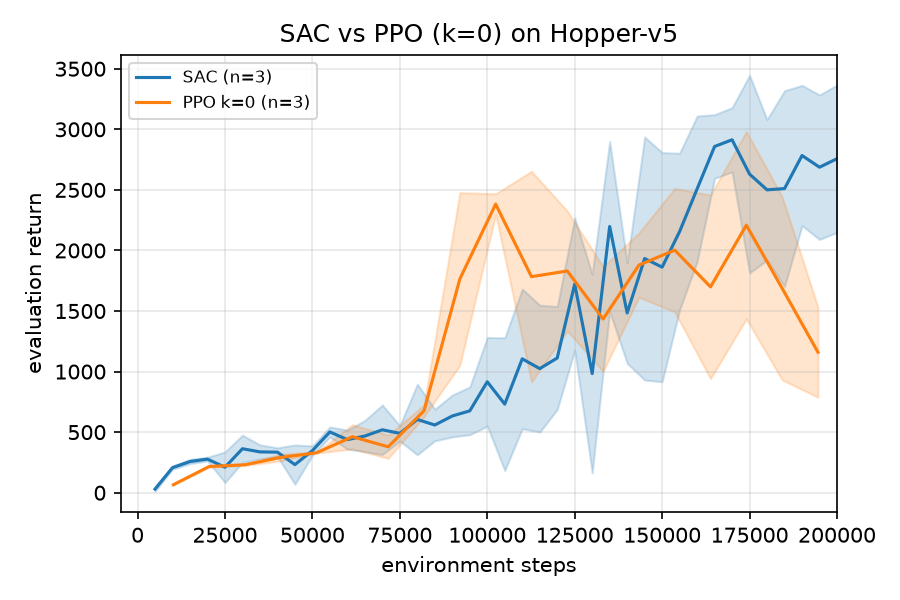
\includegraphics[width=\linewidth]{q4_return_sac_vs_ppo.png}\caption{Evaluation return.}\end{subfigure}
  \begin{subfigure}{0.49\textwidth}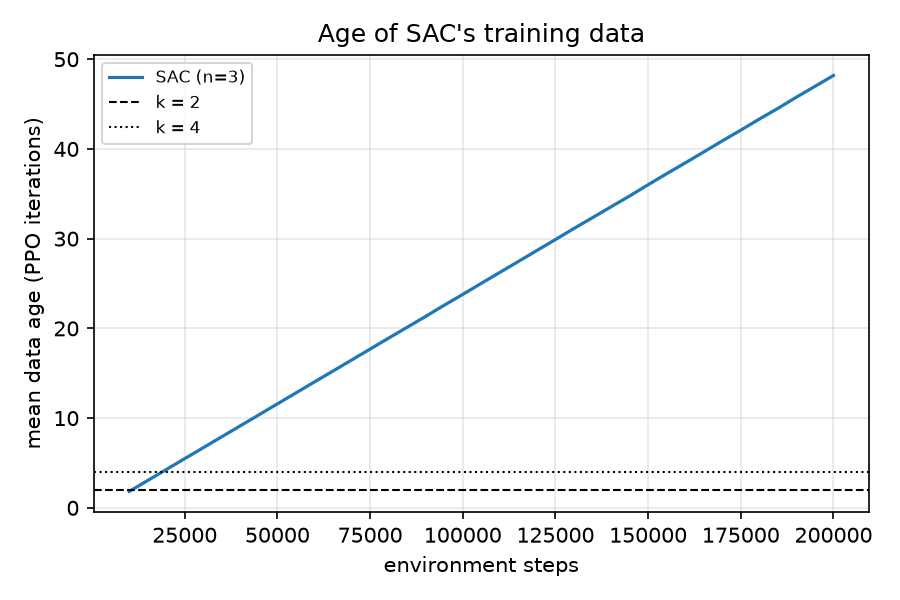
\includegraphics[width=\linewidth]{q4_data_age.png}\caption{Mean data age in PPO iterations.}\end{subfigure}
  \begin{subfigure}{0.49\textwidth}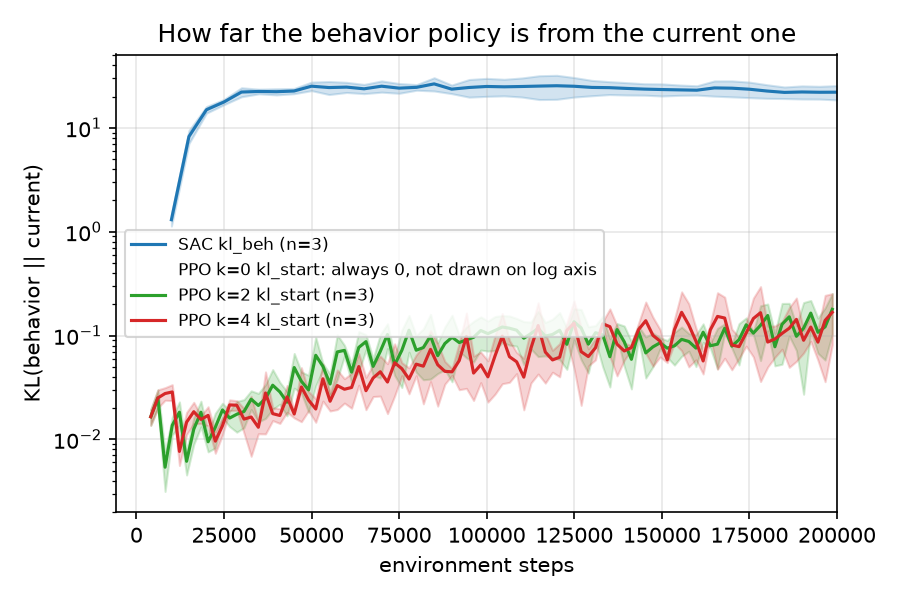
\includegraphics[width=\linewidth]{q4_kl.png}\caption{\code{kl\_beh} vs.\ PPO \code{kl\_start} (log scale).}\end{subfigure}
  \begin{subfigure}{0.49\textwidth}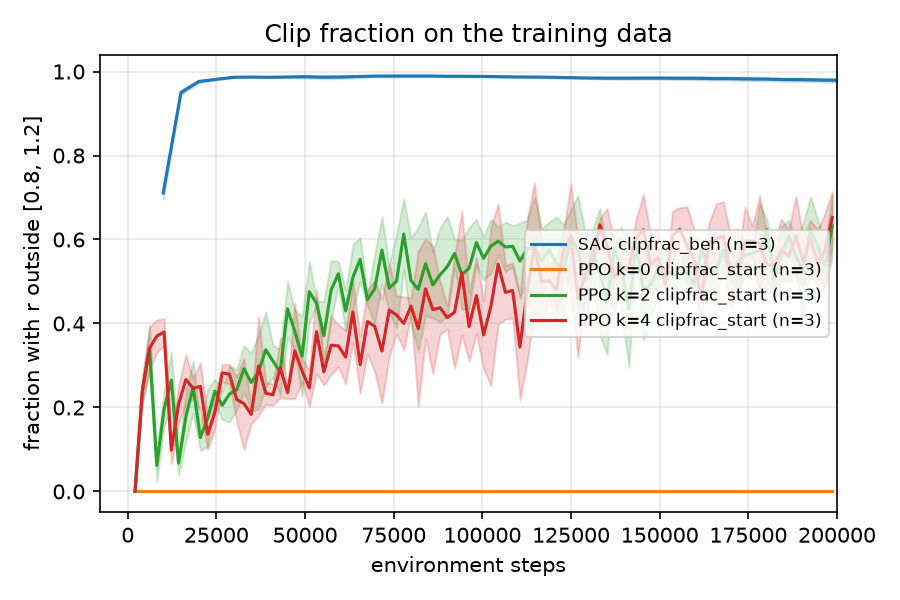
\includegraphics[width=\linewidth]{q4_clipfrac.png}\caption{\code{clipfrac\_beh} vs.\ PPO \code{clipfrac\_start}.}\end{subfigure}
  \caption{Q4(b): base SAC compared with Assignment 3 PPO. For $k=0$, PPO's \code{kl\_start} and
  \code{clipfrac\_start} are exactly 0 (the data is fresh and nothing has been updated yet), so that curve cannot be drawn on a log axis.}
  \label{fig:q4}
\end{figure}

\paragraph{The implementation works.} All three seeds of base SAC leave the 300--400 range. They first reach a
return of 1000 at 80k, 135k and 100k steps, and they end at $3240$, $3133$ and $1900$ (mean $2757\pm608$ at
$2\times10^5$). Table~\ref{tab:q4} summarizes the figures. Because PPO only logged evaluations on its own grid of
2048 steps, I compare returns as the average over the last 20k steps before each checkpoint, for both
algorithms.

\begin{table}[h]
\centering
\resizebox{\textwidth}{!}{\begin{tabular}{lcccc}
  \toprule
  & SAC (base) & PPO $k=0$ & PPO $k=2$ & PPO $k=4$ \\
  \midrule
  Return, avg.\ over 80k--100k steps   & $678\pm169$ & $1221\pm374$ & $353\pm15$ & $281\pm37$ \\
  Return, avg.\ over 180k--200k steps  & $2648\pm280$ & $1423\pm546$ & $1045\pm424$ & $556\pm209$ \\
  First reached return 1000 (per seed) & 80k, 135k, 100k & 92k, 102k, 92k & 113k, 205k, 225k & 215k, 246k, 256k \\
  KL between behavior and current policy & $\approx 22$--$25$ & $0$ & $\approx 0.10$ & $\approx 0.10$ \\
  Clip fraction on the training data   & $\approx 0.98$ & $0$ & $\approx 0.55$ & $\approx 0.55$ \\
  \bottomrule
\end{tabular}}
\caption{Q4 summary (mean $\pm$ std over seeds). KL and clip fraction for SAC are \code{kl\_beh} and
\code{clipfrac\_beh} after the first 25k steps; for PPO they are \code{kl\_start} and \code{clipfrac\_start}
averaged over 100k--200k steps. The PPO $k=2,4$ runs reached 1000 after $2\times10^5$ steps for some seeds
(they ran to $3\times10^5$ in Assignment 3).}
\label{tab:q4}
\end{table}

\begin{itemize}
  \item \textbf{Data age} (Fig.~\ref{fig:q4}b) grows in a straight line. Since nothing is ever removed and
        samples are drawn uniformly from everything collected so far, the mean age at step $t$ is about $t/2$.
        It is already $1.8$ PPO iterations at 10k steps, passes $k=4$ at about 17k steps, and reaches
        $24$ iterations at $10^5$ and $48$ iterations at $2\times10^5$ steps.
  \item \textbf{KL} (Fig.~\ref{fig:q4}c). \code{kl\_beh} jumps from $1.3$ at 10k steps to about $18$ at 25k
        steps and then stays between $22$ and $25$ for the rest of training. PPO's \code{kl\_start} is $0$ for
        $k=0$ and only about $0.01$--$0.17$ for $k=2,4$. SAC's training data is about two orders of
        magnitude further from its current policy.
  \item \textbf{Log-ratios and clip fraction} (Fig.~\ref{fig:q4}d). From 25k steps on, the median of
        $\log r_\theta$ is between $-10$ and $-14$, so the typical stored action has
        $r_\theta\approx e^{-12}\approx 6\times10^{-6}$: the current actor would almost never pick it.
        The 5th percentile is about $-70$, and even the 95th percentile is only around $0$.
        \code{clipfrac\_beh} is about $0.98$ for the whole run, compared with about $0.55$ for PPO with
        $k=2,4$ and $0$ for $k=0$.
\end{itemize}

\subsubsection*{(c) Analysis}
\paragraph{Sample efficiency.} At $10^5$ steps PPO with $k=0$ is ahead (about 1221 vs.\ 678), and it
reaches a return of 1000 a little sooner on average (about 95k vs.\ 105k steps, with SAC's seeds more spread out).
At $2\times10^5$ steps SAC is clearly ahead (about 2648 vs.\ 1423). SAC keeps improving, while PPO with
$k=0$ levels off and becomes unstable (its mean drops at the end). So in my runs SAC is slower at the start
but far more sample efficient over the full budget, and it beats every PPO lag at $2\times10^5$ steps.

\paragraph{How old is SAC's data?} The average transition SAC learns from is about $24$ PPO
iterations old at $10^5$ steps and $48$ at the end. In Assignment 3 Q5, PPO already struggled at $k=2$
(it reached 1000 about 1.2--2.4$\times$ later than $k=0$) and was much worse at $k=4$. SAC passes $k=4$
after only about 17k steps and then trains on data $10$--$25$ times older than the lag that hurt PPO, yet
it keeps learning.

\paragraph{How different is the behavior policy?} Very different. \code{kl\_beh}$\,\approx22$--$25$ is
more than 100 times PPO's \code{kl\_start}$\,\approx0.1$ at $k=2,4$. With a median ratio of about
$6\times10^{-6}$, almost every stored action is one that the current actor would essentially never choose,
and \code{clipfrac\_beh}$\,\approx0.98$ against $0.55$ for PPO. (PPO's \code{kl\_start} was an estimate from
samples, $\Ehat[(r-1)-\log r]$, while \code{kl\_beh} is the exact Gaussian KL, but both measure the
same direction, KL(behavior$\,\|\,$current), so they can be compared.) SAC's data is far more
off-policy than any data PPO could cope with.

\paragraph{If SAC used PPO's clipped loss on its replay data.} In my Assignment 3 Q5(c) answer, the samples
that are guaranteed to give an ordinary non-zero clipped gradient are the in-range ones, a fraction
$1-\code{clipfrac}$, and this is a lower bound. Here that is $1-0.98\approx2\%$ of the batch, about 5
of 256 samples. Some out-of-range samples (those with $r<0.8$ and $\Ahat>0$, or $r>1.2$ and $\Ahat<0$) would also
give a gradient, but with $r\approx10^{-5}$ the unclipped term $r\Ahat$ is tiny, and its gradient
$\Ahat\,r\,\nabla\log\pi_\theta$ is scaled by $r$ as well. So only about 2\% of the samples would give a useful signal.
SAC could not learn from its buffer the way PPO learns from its rollout.

\paragraph{What comes from the buffer and what is fresh.}
\begin{center}
\begin{tabular}{lll}
  \toprule
  Update & From the replay buffer (old policies) & Freshly sampled from current $\pi_\theta$ \\
  \midrule
  Critic & $s$, $a$, $r$, $s'$, $d$ & $a'\sim\pi_\theta(\cdot\mid s')$ and $\log\pi_\theta(a'\mid s')$ in the target \\
  Actor  & $s$ only & $\tilde a\sim\pi_\theta(\cdot\mid s)$ and $\log\pi_\theta(\tilde a\mid s)$ \\
  Temperature & (states $s$, through $\tilde a$) & $\log\pi_\theta(\tilde a\mid s)$ \\
  \bottomrule
\end{tabular}
\end{center}
The stored action $a$ appears in only one place: the left-hand side $Q_\phi(s,a)$ of the critic
regression. Every action whose \emph{probability} matters (the action at $s'$ in the target and the
action in the actor loss) is drawn from the current policy.

\paragraph{My guess.}
 My guess is that SAC can get away without the importance ratio because it never uses the old
 policy's actions to judge the current policy. A stored transition $(s,a,r,s')$ is only used as a fact
 about the environment: once $s$ and $a$ are fixed, the reward and the next state are produced by the
 environment, not by the policy, so the transition stays valid for every later policy. Whenever the
 current policy matters, SAC samples a fresh action from it and asks the critic how good that action
 is. PPO instead judges the current policy using actions that the old policy chose, so it needs the
 ratio $r$ to reweight those actions, and that only works while the two policies stay close.\\

\noindent The importance ratio exists to correct for actions that were chosen by a different policy. SAC never
needs to know how likely a stored action was. The critic learns $Q(s,a)$ for \emph{any} action:
the transition $(s,a,r,s')$ is a fact about the environment, and it is valid whichever policy chose $a$,
while the policy being evaluated only enters through the fresh $a'$. The actor is then improved
by asking the critic about fresh actions from the current policy. So the only thing that is still
``off-policy'' is the state distribution (states come from old policies), and SAC simply accepts that,
just as PPO accepts $w_\theta(s)\approx1$. My guess is that if either fresh action is replaced by a stored one, SAC
will lose its ability to use old data.

%---------------------------------------------------------------------
\subsection*{Q5: Replacing fresh actions with stored ones}

\subsubsection*{(a) Modification of the critic target}
\begin{itemize}
  \item \textbf{Buffer.} Three new arrays per transition: \code{next\_act} ($a'_b$),
        \code{next\_beh\_logp\_a} ($\log\pi_b(a'_b\mid s')$) and a flag \code{has\_next}. \code{add()} sets
        \code{has\_next = 0}, and a new method \code{set\_next(i, a, logp)} fills in the three values for position $i$.
  \item \textbf{Training loop.} I keep \code{prev\_idx}, the buffer position of the previous transition of
        the current episode. Each step, right after the agent picks its action $a$ (and before
        \code{env.step}), I call \code{buffer.set\_next(prev\_idx, a, beh\_logp\_u - tanh\_log\_det\_jacobian(u))}.
        That is the squashed behavior log-density, with the tanh term subtracted as in the
        notation section. After storing the new transition, \code{prev\_idx} is set to its position, or to
        \code{None} if the episode ended (terminated or truncated), so no action is ever linked across episodes.
        For warm-up actions this gives $\log\pi_b=-3\log2$, the uniform density, as it should.
  \item \textbf{Target.} In \code{critic\_loss} I still draw $a'\sim\pi_\theta(\cdot\mid s')$ once. With
        \code{--target-action replay}, \code{torch.where(has\_next, ...)} replaces $a'$ and
        $\log\pi_\theta(a'\mid s')$ by $a'_b$ and $\log\pi_b(a'_b\mid s')$ wherever the next action exists.
        Otherwise it falls back to the fresh sample. This covers the time-limit cut and the
        most recent transition, whose next action has not been chosen yet. For terminal transitions the
        value does not matter, since $d=1$.
\end{itemize}

\paragraph{Whose value does the critic learn?}
The target now follows the action the \emph{behavior} policy took at $s'$, and its entropy bonus
uses $\pi_b$. This is a SARSA-style target, so the critic learns the soft Q-function of the behavior policy, not of $\pi_\theta$. Because the
buffer mixes data from all past policies (including the uniform warm-up), it is the value of an average of
the old policies that filled the buffer, weighted by how much data each one contributed.

\paragraph{Which approximation from Assignment 3 Q3(b) comes back?}
The second one: using the value of the old policy in place of the current one,
$Q^{\pi_\theta}\approx Q^{\pi_b}$ (Assignment 3: $A^{\pi_\theta}\approx A^{\pi_{\theta_{\mathrm{old}}}}$).
The actor still maximizes this critic with fresh actions, so it improves the policy against the value of
older and worse policies. The state-distribution approximation $w_\theta(s)\approx1$ was already there in base SAC
and is unchanged.

\subsubsection*{(b) Modification of the actor loss}
With \code{--actor-loss naive} or \code{clip}, \code{actor\_loss(obs, batch)} does the following:
\begin{enumerate}[nosep]
  \item One call \code{self.actor.sample(obs)} gives a fresh reparameterized $\tilde a$ and $\log\pi_\theta(\tilde a\mid s)$.
  \item Under \code{no\_grad}: $\Ahat=\min_jQ_{\phi_j}(s,a)-\min_jQ_{\phi_j}(s,\tilde a)$ with the online critics and the
        stored action $a$, then $\Ahat\leftarrow(\Ahat-\mathrm{mean})/(\mathrm{std}+10^{-8})$, the same
        line as in my Assignment 3 \code{buffer.py}.
  \item $\log\pi_\theta(a\mid s)$ is replaced by \code{actor.log\_prob\_u(obs, u)} with the stored $u$.
        This is allowed because the tanh term does not depend on $\theta$.
  \item \textbf{naive:} $-\mathrm{mean}[\log\mathcal N_\theta(u\mid s)\Ahat]+\alpha\,\mathrm{mean}[\log\pi_\theta(\tilde a\mid s)]$.
  \item \textbf{clip:} $\log r_\theta=\log\mathcal N_\theta(u\mid s)-$\code{beh\_logp\_u}, $r_\theta=e^{\log r_\theta}$,
        loss $=-\mathrm{mean}[\min(r_\theta\Ahat,\mathrm{clip}(r_\theta,0.8,1.2)\Ahat)]+\alpha\,\mathrm{mean}[\log\pi_\theta(\tilde a\mid s)]$.
        \code{clipfrac\_actor} is the fraction with $\log r_\theta\notin[\log0.8,\log1.2]$ and is added to the
        returned statistics.
  \item The method still returns $\log\pi_\theta(\tilde a\mid s)$ of the fresh sample, so the temperature
        update is unchanged. The critic update is unchanged as well. Warm-up samples are kept in the actor batch,
        since their \code{beh\_logp\_u} is the exact density of the uniform policy.
\end{enumerate}
I also made \code{train.py} stop a run cleanly (writing \code{diverged.txt} with the step) if
\code{update()} ever returns a non-finite value, so that a diverging configuration still leaves a valid CSV.

\paragraph{Which part comes from the behavior policy and which from the current policy?}
\begin{itemize}
  \item \textbf{reparam:} only the states $s$ come from the behavior policies. The actions $\tilde a$, their
        log-probabilities and the gradient path through $Q(s,\tilde a)$ all come from the current policy.
  \item \textbf{naive:} the states \emph{and} the actions $a$ in the policy-gradient term come from the behavior
        policies, and nothing corrects for that. The current policy enters only through
        $\nabla\log\pi_\theta(a\mid s)$ at those stored actions, through the baseline $\Qbar(s,\tilde a)$ in
        $\Ahat$ and through the entropy term.
  \item \textbf{clip:} states and actions come from the behavior policies as in naive, but the ratio
        $r_\theta=\pi_\theta/\pi_b$ reweights the stored actions towards the current policy (clipped to
        $[0.8,1.2]$). The baseline and the entropy term again use fresh $\tilde a$.
\end{itemize}
In all three the critic itself is trained as in base SAC (fresh $a'$), so it estimates $Q^{\pi_\theta}$.

\subsubsection*{(c) Results}
\begin{figure}[h]
  \centering
  \begin{subfigure}{0.49\textwidth}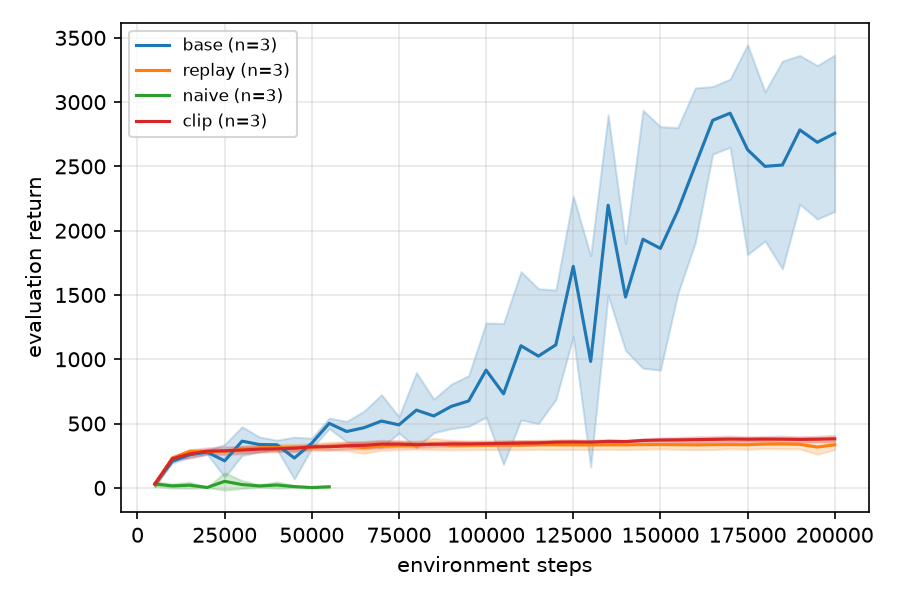
\includegraphics[width=\linewidth]{q5_return.png}\caption{Evaluation return.}\end{subfigure}
  \begin{subfigure}{0.49\textwidth}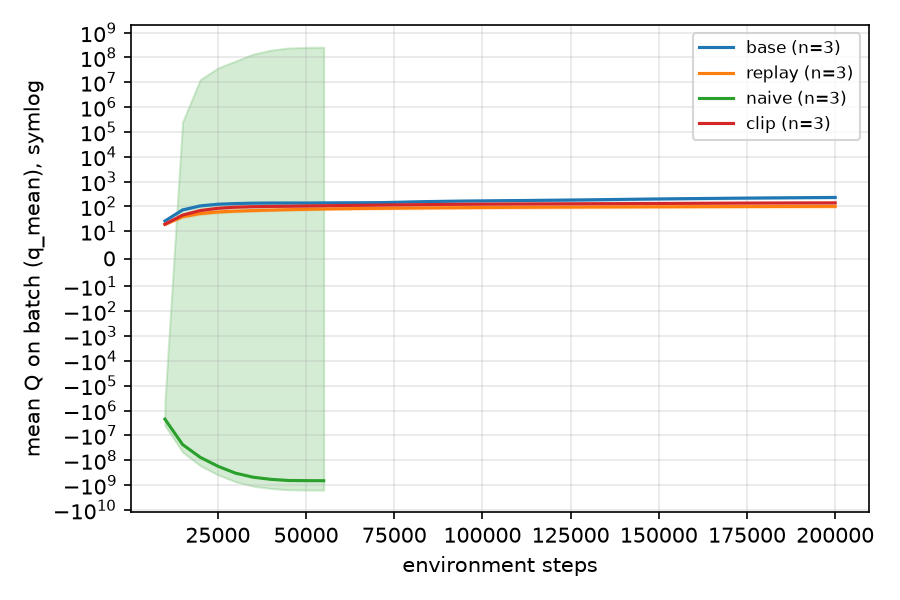
\includegraphics[width=\linewidth]{q5_q_mean.png}\caption{\code{q\_mean}.}\end{subfigure}
  \begin{subfigure}{0.49\textwidth}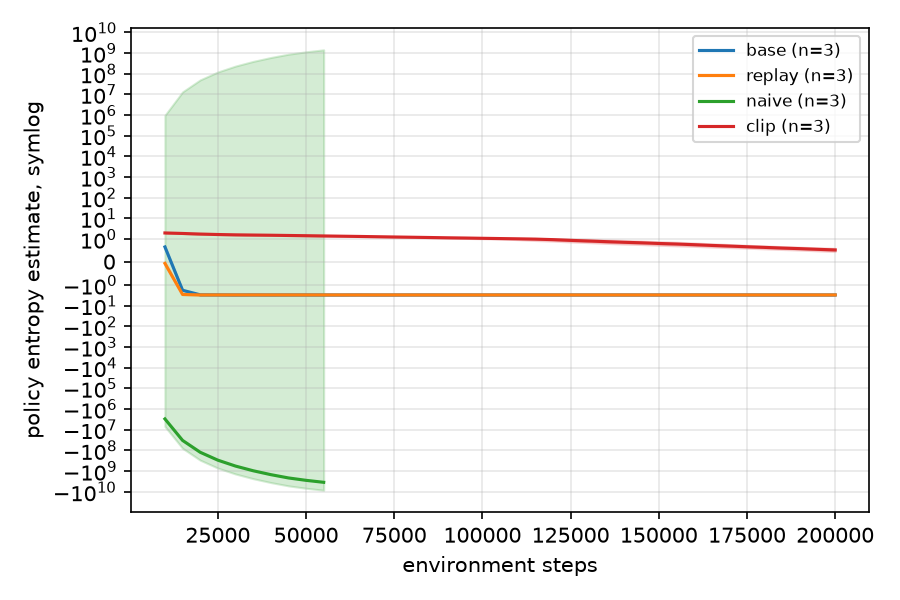
\includegraphics[width=\linewidth]{q5_entropy.png}\caption{\code{entropy}.}\end{subfigure}
  \begin{subfigure}{0.49\textwidth}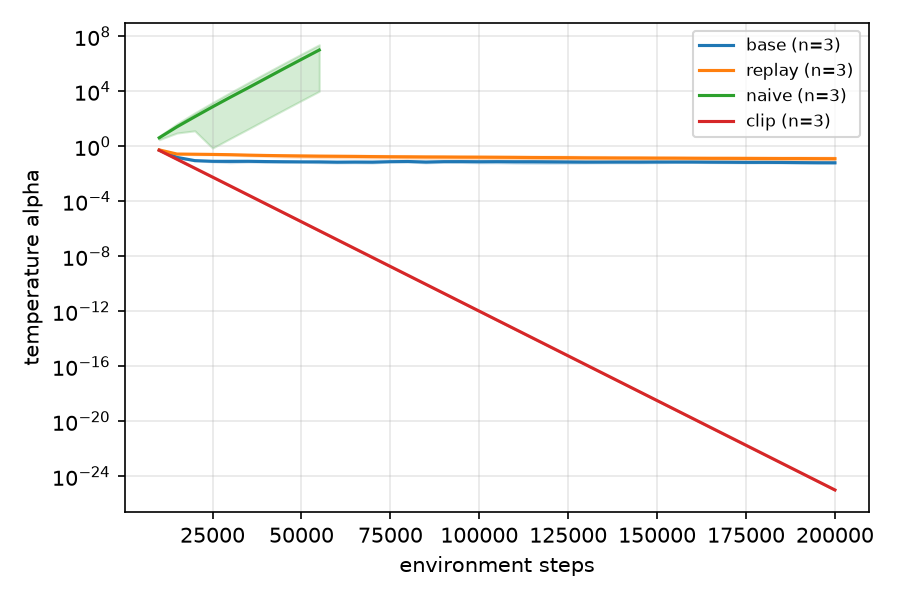
\includegraphics[width=\linewidth]{q5_alpha.png}\caption{\code{alpha} (log scale).}\end{subfigure}
  \caption{Q5(c): the four configurations. \code{q\_mean} and \code{entropy} use a symmetric log axis
  (linear near 0), because naive reaches values around $\pm10^9$. The naive curves stop at 55k steps, the
  last evaluation that all three seeds reached (see text).}
  \label{fig:q5}
\end{figure}
\begin{figure}[h]
  \centering
  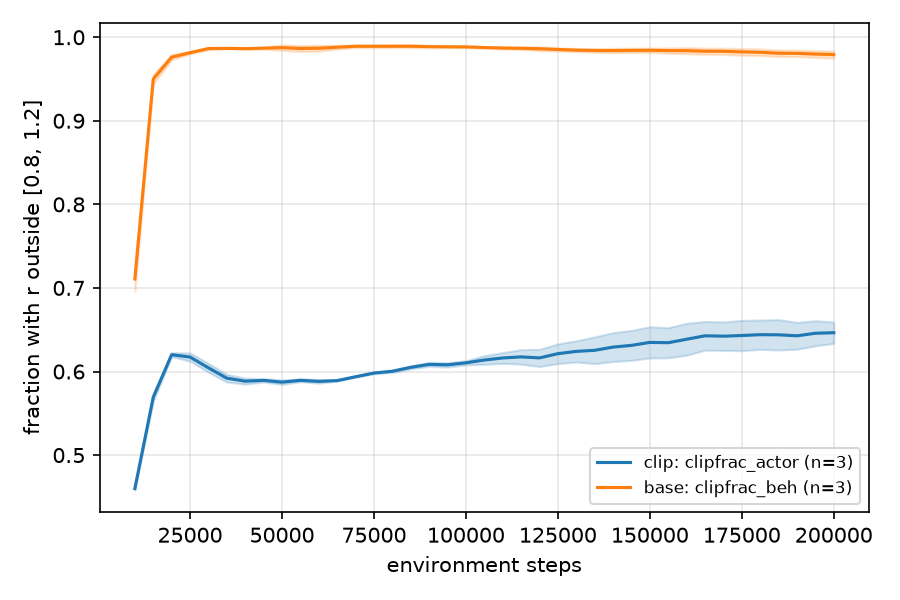
\includegraphics[width=0.55\textwidth]{q5_clipfrac.png}
  \caption{\code{clipfrac\_actor} of the clip configuration and \code{clipfrac\_beh} of base.}
  \label{fig:q5clip}
\end{figure}

\begin{table}[h]
\centering
\resizebox{\textwidth}{!}{\begin{tabular}{lcccc}
  \toprule
  At $2\times10^5$ steps & base & replay & naive & clip \\
  \midrule
  Evaluation return   & $2757\pm608$ & $335\pm37$ & diverged (2--50) & $382\pm25$ \\
  \code{q\_mean}      & $230\pm11$ & $101\pm9$ & $\sim -10^{9}$ & $139\pm7$ \\
  \code{entropy}      & $-3.00$ & $-3.00$ & $-10^{10}$ (seed 1), $\approx-25$ (seeds 2, 3) & $0.53\pm0.07$ \\
  \code{alpha}        & $0.064$ & $0.128$ & $10^{7}$--$10^{15}$ & $\approx10^{-24}$ \\
  \code{clipfrac\_actor} / \code{clipfrac\_beh} & $0.98$ (beh) & -- & -- & $0.65$ (actor) \\
  \bottomrule
\end{tabular}}
\caption{Q5 summary (mean $\pm$ std over seeds; naive is given at the step where each seed stopped).}
\label{tab:q5}
\end{table}

\begin{itemize}
  \item \textbf{base} learns to $2757\pm608$. Its entropy sits at the target $-3$, with $\alpha\approx0.06$--$0.08$.
  \item \textbf{replay} stays at the ``standing still'' level: about 300--390 for every seed during the whole run
        ($335\pm37$ at the end). Its \code{q\_mean} is less than half of base's ($101$ vs.\ $230$) and grows much more slowly.
        Entropy is at the target and $\alpha\approx0.13$.
  \item \textbf{clip} is also stuck, at $382\pm25$. Its entropy never comes down to the target: it starts around
        $2$ and is still $0.53$ at the end. Because the entropy stays above the target the whole time, the temperature update
        keeps lowering $\alpha$, which falls in a straight line on the log plot to about $10^{-24}$.
        \code{clipfrac\_actor} is $0.59$--$0.65$, lower than base's \code{clipfrac\_beh}$\,\approx0.98$ but still most of the batch.
  \item \textbf{naive became numerically unstable in all three seeds}: the update returned non-finite values at
        steps \textbf{55,825}, \textbf{142,133} and \textbf{147,727} (seeds 1, 2, 3), and the runs stopped there.
        Long before that it had already failed. The return was about 5 for seed 1 and jumped between 1 and about 150 for
        seeds 2 and 3 (the hopper falls almost at once). Within 10k steps of learning the entropy estimate fell to about
        $-10^{7}$ (seed 1) and $-10^{5}$ (seeds 2, 3). For seed 1 it kept falling to $-10^{10}$; for seeds 2 and 3 it
        came back up to about $-25$, but never to the target $-3$. $\alpha$ grew without stopping, to between $10^{7}$ and
        $4\times10^{15}$, and \code{q\_mean} fell to about $-10^{9}$.
        In seed 1 the last update had \code{critic\_loss}$\,=\infty$ and \code{clipfrac\_beh}$\,=1$.
        The plots use the data up to 55k steps, the last evaluation all three seeds share.
\end{itemize}

\subsubsection*{(d) Analysis}
\paragraph{Ranking.} base $\gg$ clip $\gtrsim$ replay $\gg$ naive. Only base learns to hop. clip and replay are stable
but stay at the standing level (clip is slightly higher at the end, but the gap is small compared with the
gap to base). naive diverges. Each change replaces exactly one fresh action with a stored one, so the
gap between base and the others shows that \emph{both} fresh actions are needed.

\paragraph{replay: the critic learns the value of the old policies.}
Only the critic changes. With the stored next action in the target, the critic no longer answers ``how good
is this action if I then follow my \emph{current} policy?'' but ``how good is it if I then act like my
\emph{old} policies?''. The actor improves against that, so it only learns to be a little better than the old
data. When the actor gets better, the critic does not give it credit, so improvements cannot build on each
other. \code{q\_mean} agrees: $101$ for replay against $230$ for base at the end. This is
$A^{\pi_\theta}\approx A^{\pi_{\theta_{\mathrm{old}}}}$ from Assignment 3 Q3(b), with an ``old'' policy up to 48
PPO iterations old.

\paragraph{naive: the wrong actions, and nothing to stop the push.}
The policy-gradient term should use actions from the current policy, but naive uses the stored actions from
old policies, with no $r_\theta$ to correct for this (as in Assignment 3 Q6). With a median $r\approx10^{-5}$,
these are actions the current policy would almost never take.

Worse, with fixed actions the loss $-\Ehat[\log\pi_\theta(a\mid s)\Ahat]$ has no floor. For a bad action
($\Ahat<0$) the actor can keep lowering the loss by moving its mean further away from that action, forever.
Good actions cannot balance this, because their probability cannot grow past a limit. So the mean runs off,
tanh saturates, every action sits at $\pm1$ and the hopper falls (return near 0). The entropy then crashes
($-10^5$ to $-10^{10}$), $\alpha$ keeps growing to push it back up (up to $\sim10^{15}$), and in the end the
critic target overflows and the run stops. In Assignment 3 with $k=0$ this did not happen, because the actions
were fresh and thrown away after each iteration. Here the same stored actions are pushed against for the whole run.

\paragraph{clip: correct, but too little signal.}
The ratio $r_\theta$ fixes naive's problem. It gives little weight to stored actions the current policy would
rarely take, so the update is about the current policy again, and clipping stops the runaway (once $r<0.8$ on
a bad action, the push stops). But this costs most of the signal:
\begin{itemize}[nosep]
  \item Only $35$--$40\%$ of the samples are inside the clip range (\code{clipfrac\_actor}$\,=0.59$--$0.65$). The
        rest give no gradient, or one that pulls the policy back towards the old data.
  \item To keep samples in range, the policy has to stay broad and close to the old data (entropy $0.5$--$2$,
        far above the target $-3$; $\alpha$ falls to $10^{-24}$). Staying close to the old data is exactly what
        stops it from improving, so the hopper only stands.
\end{itemize}
reparam does not have this problem. It asks the critic directly which way to move its own fresh action to raise
$Q$, so every sample gives a useful gradient, with no ratio and no clipping.

\paragraph{Back to my guess from Q4(c).} The guess was right. SAC gets away without an importance ratio because the
only behavior-policy data it uses are the states and the transitions $(s,a,r,s')$. A transition is a fact about the
environment, valid whichever policy chose $a$, and $Q(s,a)$ can be fitted to it for any $a$. Everything that depends
on \emph{which} policy is being evaluated or improved, the action at $s'$ in the target and the action in the actor
loss, is sampled fresh from $\pi_\theta$. When I replaced either fresh action with the stored one, SAC stopped learning
(replay, clip) or diverged (naive). SAC can do this because its critic is an action-value function: it can be asked
about any action, including ones the current policy has never tried, so fresh actions can be evaluated without being
executed. PPO cannot do the same. Its critic $V(s)$ says nothing about individual actions, and its advantages come from
GAE, which needs the rewards that actually followed the stored action along the behavior trajectory. Advantages
therefore exist only for actions that were actually taken, so PPO must reuse those actions and reweight them with $r_\theta$,
which only works while the policies are close. That is why it clips and throws its data away after every iteration.

\paragraph{What each algorithm gains and pays.}
\begin{itemize}[nosep]
  \item \textbf{PPO} gains simplicity and stability. It needs only $V(s)$, its gradient is close to the true on-policy
        gradient, and each run took only 5--15 minutes in Assignment 3. It pays in data: every rollout is used for one
        iteration and then thrown away, and even a lag of $k=2$ slows learning (Assignment 3 Q5). At $2\times10^5$ steps it
        is well behind SAC.
  \item \textbf{SAC} gains the ability to learn from all of its data, including transitions 48 iterations old with
        $\mathrm{KL}\approx22$, which gives much better returns at $2\times10^5$ steps. It pays with a learned
        $Q(s,a)$ that must be accurate. It needs twin critics, target networks and one update per environment step, which costs much more
        computation (about 3.5 hours per run here with 12 runs in parallel, compared with minutes for PPO). It was
        slower early in my runs and varied more between seeds. It also still ignores the state-distribution mismatch
        ($w_\theta(s)\approx1$), just as PPO does.
\end{itemize}

\end{document}
